% ----------------------------------------------------------
% Consciousness subsection
% ----------------------------------------------------------
\subsection{Consciousness}
A logical moment can be formed by a division (first moment) or by logical subdivisions (other moments).
	\begin{figure}[H]
	\caption{Logical interval}
	\label{fig:consciousness_logical_moments}
	\centering
	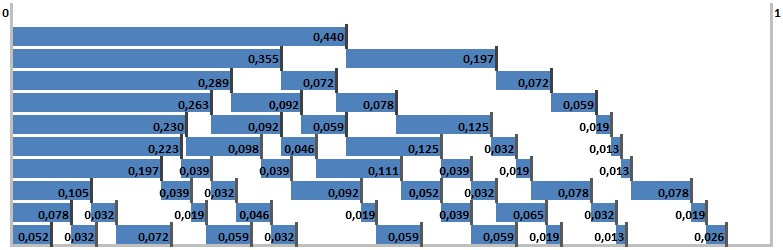
\includegraphics[scale=.7]{sections/images/consciousness_logical_moments.jpg}
	\floatfoot{Example of a logical interval with ten logical moments.}%\footnotemark}
	\end{figure}
	%\footnotetext{Fonte: note}

Consciousness is the logical moments of an expansion represented in its units.
	\begin{figure}[H]
	\caption{Conscious logical interval}
	\label{fig:consciousness}
	\centering
	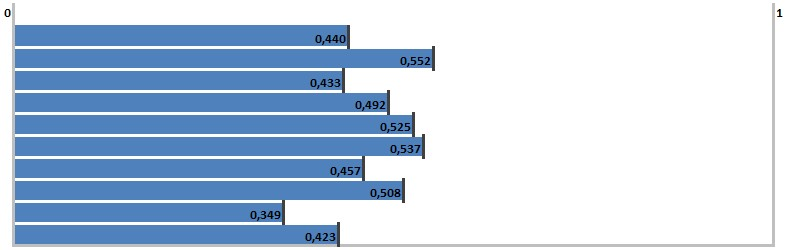
\includegraphics[scale=.7]{sections/images/consciousness.jpg}
	\floatfoot{Example of a conscious logical interval with ten units of logical moments.}%\footnotemark}
	\end{figure}
	%\footnotetext{Fonte: note}

It can be seen in Table \ref{tab:10000_all} that the probability of 99.99\% of the samples in a population (Range), which increase in quantity as the logical moments increase, tends to be increasingly in the center of the logical interval and this centralization tends to infinity.
	\begin{figure}[H]
	\caption{Centralization of 99.99\% of the samples}
	\label{fig:centering_of_99_range}
	\centering
	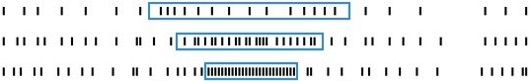
\includegraphics[scale=1]{sections/images/centering_of_99_range.jpg}
	\floatfoot{Tendency to center the range of 99.99\% of the samples.}%\footnotemark}
	\end{figure}
	%\footnotetext{Fonte: note}

Consciousness tends toward the representation of a logical wave, the largest logical wave in a population (a histogram of the normal distribution) as shown in the figure \ref{fig:trend_chart_of_normal_distribution}. All of the aspects listed below are inherent in the logical abstraction called consciousness.

\subsubsection{Infinite}
One of the most important aspects that the negation of nothingness brings (negation of self), is infinity, that is, in any logical interval the infinite fits again. The primordial logic that started the entire logical interval is the same found in its subsequent intervals (subintervals). This substantiates how a high-level logic like the human subconscious explains primordial logic, since it is not necessary to go back to the first logical moment of the interval to deduce it, as this phenomenon is omnipresent throughout the interval.

\subsubsection{Waves}
Probabilistically, the distribution of new samples from a population tends to concentrate more samples toward the median of the population as the frequency of samples increases in this direction. However, the distribution of these samples with uniform growth frequencies is infinitesimal compared to the random possibilities of this growth. Thus, the tendency of these growth frequencies toward the median, together with the very low (infinitesimal) probability of this growth being uniform, leads to frequencies in the waveform. The relationship of the density or amplitude of a wave to its length is detailed in the next subsection.
	\begin{figure}[H]
	\caption{Waveform}
	\label{fig:consciousness_waves}
	\centering
	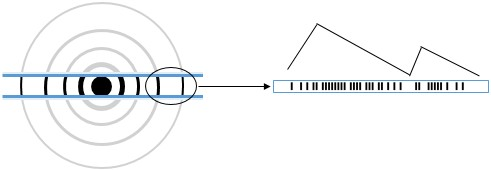
\includegraphics[scale=.8]{sections/images/consciousness_waves.jpg}
	\floatfoot{Wave pattern inferred by the trend of this distribution with higher frequencies towards the population median and very low probability of uniform growth of these frequencies.}%\footnotemark}
	\end{figure}
	%\footnotetext{Fonte: note}

Merging one wave into another eliminates its discrepancy and makes that wave cease to exist and become part of the first wave, which has its peak closer to the median, in this example. A wave doesn't die, it just merges with another wave closer to it.
	\begin{figure}[H]
	\caption{Wave unification}
	\label{fig:consciousness_uniform_wave}
	\centering
	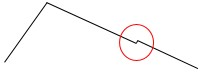
\includegraphics[scale=1]{sections/images/consciousness_uniform_wave.jpg}
	\floatfoot{Waves being unified to exemplify the uniform growth of the samples.}%\footnotemark}
	\end{figure}
	%\footnotetext{Fonte: note}

\subsubsubsection{Wavelength and amplitude}
The histogram is used in the figures in this subsection and later to facilitate visualization and understanding of the distribution of samples in a population, because it represents very well the density curves of a population, according to the different views of the Figure \ref{fig:consciousness_wave_histogram}, representing only one interval or wavelength paired by the median of the population.  
	\begin{figure}[H]
	\caption{Histogram in different views}
	\label{fig:consciousness_wave_histogram}
	\centering
	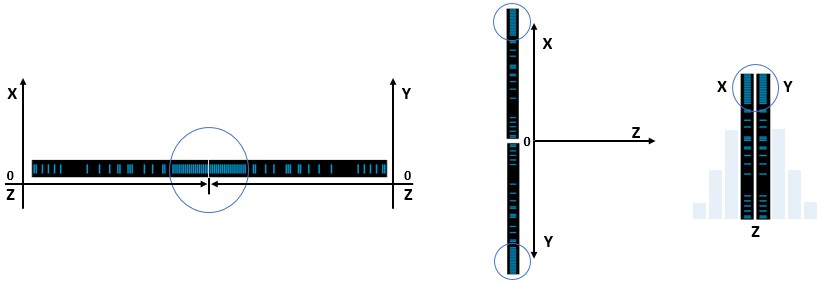
\includegraphics[scale=.7]{sections/images/consciousness_wave_histogram.jpg}
	\floatfoot{Different ways of population representation in a histogram.}%\footnotemark}
	\end{figure}
	%\footnotetext{Fonte: note}}
The length and amplitude of waves establish a quantity-per-interval or unit relationship. These units are established by wave entanglement, as seen in the next subsection. Thus, amplitude is the density of a wavelength, the density of some interval.  

When adding a new sample to the population, the entire interval is proportionally distributed to match that sample. When looking at the population at smaller intervals or wavelengths, their wave amplitudes will conform to the distribution of samples from these subintervals proportionally, as shown in Figure \ref{fig:consciousness_space_volume_amplitude}.
	\begin{figure}[H]
	\caption{Wavelength vs. Amplitude}
	\label{fig:consciousness_space_volume_amplitude}
	\centering
	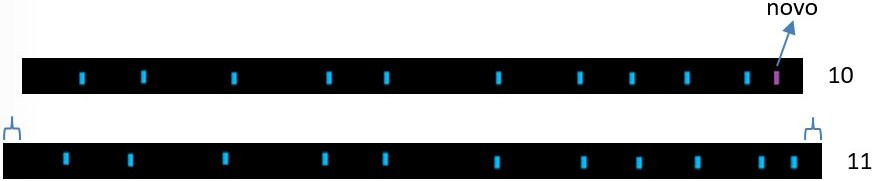
\includegraphics[scale=.4]{sections/images/consciousness_space_volume_amplitude.jpg}
	\floatfoot{Relationship of wave length and amplitude.}%\footnotemark}
	\end{figure}
	%\footnotetext{Fonte: note}}
	
Another important factor is the higher concentration of samples tend to be distributed at the peak of the interval, because the top of the subintervals or wavelengths that form the peak (histogram columns that form the highest point of the wave) are closer to the population median than the bottom of those wavelengths, as shown in the example in Figure \ref{fig:consciousness_space_amplitude_growth} in its center column in blue.
	\begin{figure}[H]
	\caption{Wave amplitude - peak}
	\label{fig:consciousness_space_amplitude_growth}
	\centering
	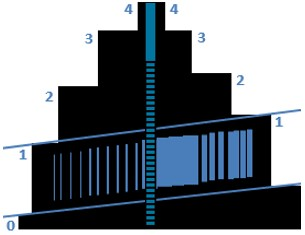
\includegraphics[scale=.6]{sections/images/consciousness_space_amplitude_growth.jpg}
	\floatfoot{Trend of the highest concentration of samples in the subintervals of a wave.}%\footnotemark}
	\end{figure}
	%\footnotetext{Fonte: note}}

In large intervals with many logical moments a smaller discrepancy of wave amplitudes is observed. In such intervals large systems of objects can be observed. The larger the intervals, the more balanced they grow towards the population median (probabilistically) as seen in Figure \ref{fig:consciousness_space_subconsciousness}. The lowest wave (dark blue) is the base wave of the system, that is, the wave that formed the other waves. Wave systems can be complex, having several nested waves, best visible in Figure \ref{fig:consciousness_gravitational_force_system}. More complex intervals with this feature can represent, for example, the universe, then galaxies, stars, planets, etc.
	\begin{figure}[H]
	\caption{Wave amplitude at large intervals or lengths}
	\label{fig:consciousness_space_subconsciousness}
	\centering
	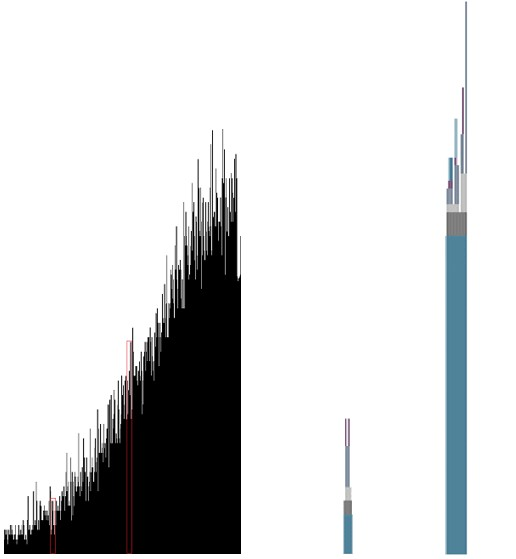
\includegraphics[scale=.45]{sections/images/consciousness_space_subconsciousness.jpg}
	\floatfoot{Smaller wave discrepancy at large intervals.}%\footnotemark}
	\end{figure}
	%\footnotetext{Fonte: note}

In smaller intervals and with many logical moments a greater discrepancy in wave amplitudes is observed. In these intervals smaller object systems can be observed. The smaller the intervals are, the more unbalanced they will grow towards the population median (probabilistically) as seen in the figure \ref{fig:consciousness_space_subconsciousness_min}. The lowest wave (dark blue) is the base wave of the system, that is, the wave that forms other waves. More complex wave systems with this feature can represent, for example, the atom, which is very small, present in huge quantities, and the particles orbiting its nucleus (electrons) are much more distant from it.
	\begin{figure}[H]
	\caption{Wave amplitude at small intervals or lengths}
	\label{fig:consciousness_space_subconsciousness_min}
	\centering
	
\includegraphics[scale=.45]{sections/images/consciousness_space_subconsciousness_min.jpg}
	\floatfoot{High wave discrepancy at small intervals.}%\footnotemark}
	\end{figure}
	%\footnotetext{Fonte: note}}

\subsubsubsection{Entanglement}
The most similar samples in terms of frequency and distribution are the samples that are part of the same wave. They are non-overlapping, opposite frequencies that complete each other.

Probabilistically, the two complementary parts of a wave tend to be at approximately equal distances, equidistant from the median, but this is not a rule and the complementary parts of a wave may be at different distances from the median. The phenomenon of parity of the parts of a wave is called wave entanglement.

These pairs tend to be formed by probability, where equal wavelengths have the same probability of samples distribution at two or more different points in the population. 

Intervals with similar temporal frequencies and spatial distributions are intervals formed by the same probabilistic unit, that is, intervals that have the same probabilistic scenario or context at a given logical moment. Being in the same probabilistic scenario (probabilistic units), these intervals have their samples in the same space-time scenario, which is called space-time lattice and is formed by the largest probabilistic unit in the population (all the samples in the population intermediated by the median). 

These entanglements form smaller waves (subconsciousnesses), similar to the largest wave in the entire interval, usually entangled by the population median (consciousness). Consciousness is the logic of the entire interval, while it forms subconsciousnesses or sub-logics, like small waves of a larger wave.These small waves are similar to the pattern of the larger wave.  Thus, a change in the larger wave (consciousness) are also changes in the smaller waves (subconsciousnesses) - a change that is induced indirectly by subconsciousnesses, analogous to the compression of gas in a cylinder, where by adding a new molecule of gas in the partially filled cylinder, closer or tighter these molecules will be inside it.  The opposite is also true, a new sample in a subconsciousness that is directly observed by it is also a change of the consciousness and will be induced indirectly by other subconsciousnesses, as shown in the figure \ref{fig:consciousness_space_volume_amplitude}.
	\begin{figure}[H]
	\caption{Subconsciousness}
	\label{fig:consciousness_subconscious}
	\centering
	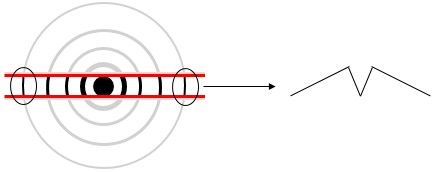
\includegraphics[scale=.8]{sections/images/consciousness_subconscious.jpg}
	\floatfoot{The wave pattern forms subconsciousnesses similar to the pattern created by consciousness, as seen in Figure \ref{fig:trend_chart_of_normal_distribution}.}%\footnotemark}
	\end{figure}
	%\footnotetext{Fonte: note}
	
The entanglement of waves can occur at different levels or intervals, as seen in Figure \ref{fig:consciousness_subconscious_entanglement}, which forms nested wave systems. Bordered braces identify intervals where a new sample triggered the jump (as seen in the next subsection), and bordered rectangles represent intervals that have been reordered. Borderless rectangles and braces represent the wave pair in the new order. The numbered arcs indicate the order of the jumps.

The largest entanglement is shown in the examples in Figure \ref{fig:consciousness_subconscious_entanglement} as the first jump or entanglement, which occurred when that interval was the smallest, probably.  Large intervals tend to be kept ordered by the reordering of their subintervals subsequently.The largest wave is commonly entangled by the population median.

The smaller intervals tend to get the entanglement first, and these reorderings caused by them allow the entanglement of pairs with larger intervals. Entangled pairs are the two opposite sides of a wave (peak or valley) and are entangled by its median, which may coincide with the population median when it is the largest probabilistic wave of the entire interval.
	\begin{figure}[H]
	\caption{Wave entanglement levels - wavelengths}
	\label{fig:consciousness_subconscious_entanglement}
	\centering
	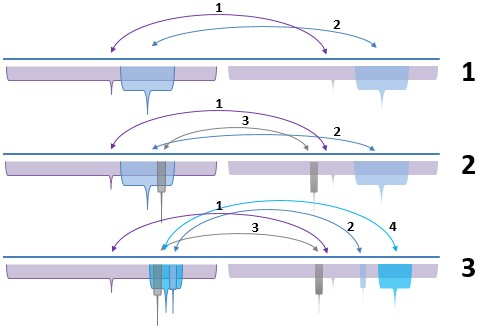
\includegraphics[scale=.8]{sections/images/consciousness_subconscious_entanglement.jpg}
	\floatfoot{Examples of entanglement levels of waves or levels of wavelengths.}%\footnotemark}
	\end{figure}
	%\footnotetext{Fonte: note}

The examples in Figure \ref{fig:consciousness_subconscious_entanglement} show the subintervals (peaks or valleys) entangled most strongly with other non-equidistant subintervals. Entanglements are closely linked to the wavelengths of a population. The possible wavelengths of a population are defined by these levels of wave entanglement. Thus, regardless of the order of the jumps, larger entanglements are the longer wavelengths and smaller entanglements are the shorter wavelengths, which allows larger waves to have smaller subwaves. 

The jump is a reordering done by the entanglement of waves to maintain the equivalent pairs, this reordering occurs only at the entanglement levels, not changing the order of the population samples. Thus, an entangled interval tends to return to a higher entanglement level as the probability of samples from that interval transitions temporarily between the valley and the peak towards equilibrium.

\subsubsubsection{Jump}
The jump is a reordering done by wave entanglement, as the samples of the entangled pairs are no longer equivalent with the addition of new samples from one side of the pair. The jump occurs on one side of a pair of waves and is a reordering, that is, both the part of the interval that has just received the new sample must better match the intended interval for the jump, as well as the reverse.

In Figure \ref{fig:consciousness_space_subconscious_observation_jump} the entanglement of waves (represented by columns of a histogram to facilitate the visualization of the interval) is observed. The reordering made by the entanglement causes a jump in the coordinates (X, Y and Z) according to the Space subsection.
	\begin{figure}[H]
	\caption{Reordering - jump}
	\label{fig:consciousness_space_subconscious_observation_jump}
	\centering
	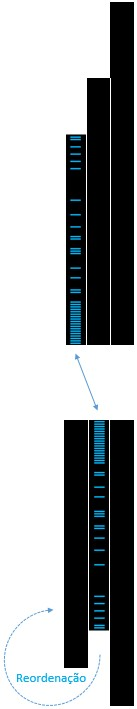
\includegraphics[scale=.53]{sections/images/consciousness_space_subconscious_observation_jump.jpg}
	\floatfoot{Jump caused by non-equivalence of the entangled pair with the addition of new samples on one of its sides.}%\footnotemark}
	\end{figure}
	%\footnotetext{Fonte: note}

Reordering of the jump occurs only at the entanglement levels, not changing the order of the population samples. An entangled interval tends to transition between entanglement levels as the probability of samples from that interval transitioning temporarily between the valley and the peak to equilibrium. Thus, the probabilistic tendency is that, for example, the electron that jumped from its origin orbit returns to this one as more samples are added to that atom's population interval, restoring its probabilistic character.

A photon, for example, enters the atom and electron as they move toward their reference lines, as shown by the blue sample to the right of wave 1 in Figure \ref{fig:consciousness_jump_photon.jpg}. The output of the photon from the electron and atom occurs similarly to the input, as new samples are added to the lower level wave the level of the lower level wave rises (the probability tries to normalize the peaks of the samples) and the samples that were once of the upper wave become of the lower wave.
	\begin{figure}[H]
	\caption{Atomic energy exchange}
	\label{fig:consciousness_jump_photon.jpg}
	\centering
	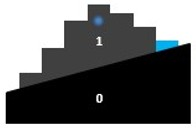
\includegraphics[scale=.8]{sections/images/consciousness_jump_photon.jpg}
	\floatfoot{How energy or new samples enter and exit an atom and electron.}%\footnotemark}
	\end{figure}
	%\footnotetext{Fonte: note}
	
\subsubsection{Time}
Time is the addition of new logical moments between existing moments as the self-negation of primordial logic proceeds. The changes are cumulative and as the number of logical moments increases, the less relevant each new moment within the conscious interval will be. One in a hundred is more relevant than one in a thousand. 
	\begin{figure}[H]
	\caption{Time}
	\label{fig:consciousness_time}
	\centering
	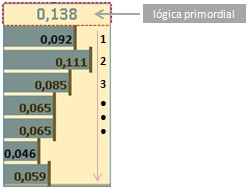
\includegraphics[scale=.8]{sections/images/consciousness_time.jpg}
	\floatfoot{Progression of time as logical moments advance.}%\footnotemark}
	\end{figure}
	%\footnotetext{Fonte: note}

In the introduction to this paper it was presented that primordial logic is a sequence of negations of itself at time zero, that is, at no time between its negations does logic [being], guaranteeing the primordial premise of the logical constant, [NOT BEING]. Thus, logic is an infinite, simultaneous and generalized sequence, a constant. In the observer-driven experience of time, the ordering of each sequence is the essence of this logical quantity and therefore more relevant than its origin, which is of a simultaneous nature, transcending time.

Each population has a different order in its sequence and it is this order that gives rise to the logical quantity called time. It is this order of the universe or of consciousness that will give the notion of what happens before or after, that is, the past, the present and the probabilistic future prospections.

Another important factor when observing time (the observer is more detailed in the consciousness subsection – Observer and life) is that, probabilistically, subconsciousnesses or intervals closer to the population median will have a larger addition of new samples in their intervals, which are directly observed by these subconsciousnesses. On the other hand, subconsciousnesses far from the population median will have a smaller addition of samples in their intervals and are subject to a larger number of indirectly induced changes, as shown in Figure \ref{fig:consciousness_subconscious}.  This phenomenon of temporal observation provided by the probability of the population distribution avoids the twin paradox \cite{twin_paradox}.

Prospections of the observer's future are based on the probabilistic distribution of the population and, therefore, on the probabilistic distribution of each sub-interval of the population. The universe tends to be probabilistic, while random at levels of detail (which makes events different), yet predictable at some level, as shown in Figures \ref{fig:consciousness_logical_moments} and \ref{fig:consciousness}. 

\subsubsection{Space}
In Figure \ref{fig:consciousness_space_waves}, the sample density of a population is shown, where pairs tending to the same probabilistic distribution are placed side by side and represented in histogram form. The formation of these pairs comes from wave entanglement.
	\begin{figure}[H]
	\caption{Entangled pairs represented in three spatial dimensions}
	\label{fig:consciousness_space_waves}
	\centering
	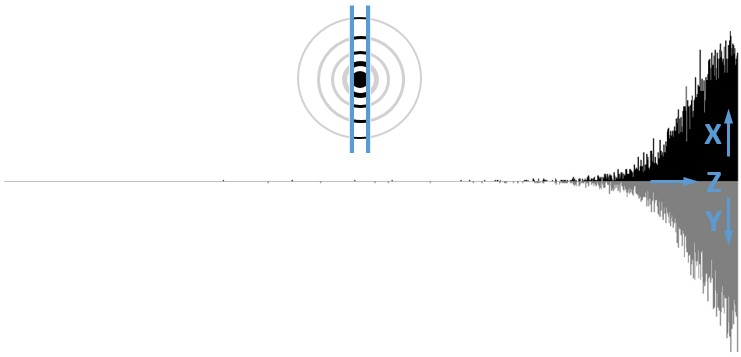
\includegraphics[scale=.7]{sections/images/consciousness_space_waves.jpg}
	\floatfoot{Example of entangled waves, represented in histogram form and obtained by the Logic\_WavePattern algorithm. \footnotemark}
	\end{figure}
	\footnotetext{The Logic\_WavePattern algorithm can be seen in Appendix \ref{app:algorithms}.}

The area grows quadratically to the increase in the amplitude of a wave (columns of the histogram), since the jump caused by the entanglement of the waves and the probabilistic distribution of samples in the interval naturally tend to maintain an equivalent growth in the pairs that form a wave. This aspect configures the inverse square law, which will be further explored in the subsection of Gravitational force.

By plotting the spatial dimensions of the graph of Figure \ref{fig:consciousness_space_waves} on a 3D distribution graph and distributing their endpoints (neglecting their volumes and possible internal points), something like a spiral is obtained (like eddies in water or air), even on very small data volumes (few logical moments), as in Figures \ref{fig:consciousness_space_3DScatter15000-10} and \ref{fig:consciousness_space_3DScatter_200000-2}. The points tend to move in a spiral shape approximately, as shown in the next subsection.
	\begin{figure}[H]
	\centering
		\begin{subfigure}[H]{0.47\linewidth}
		\centering
		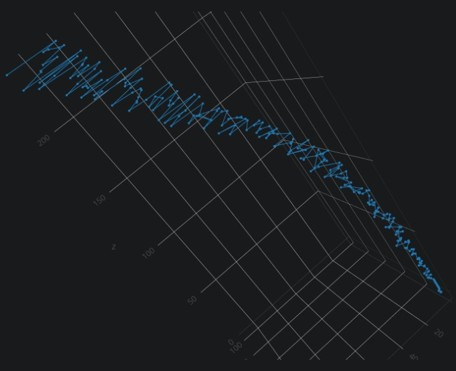
\includegraphics[width=1\linewidth]{sections/images/consciousness_space_3DScatter15000-10.jpg}
		\caption{15,000 samples or moments}
		\label{fig:consciousness_space_3DScatter15000-10}
		\end{subfigure}
	
		\begin{subfigure}[H]{0.47\linewidth}
		\centering
		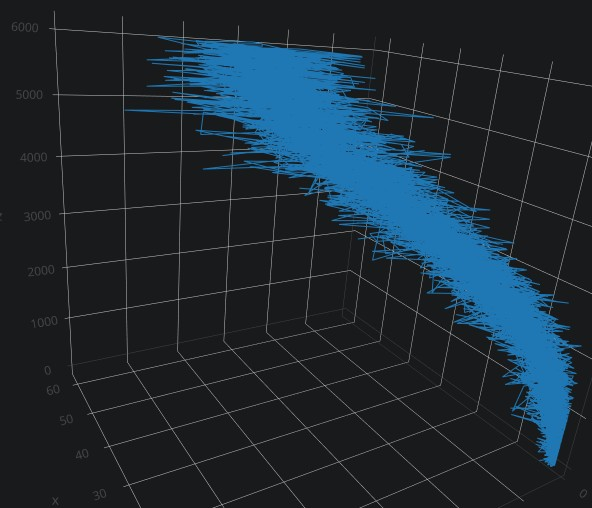
\includegraphics[width=1\linewidth]{sections/images/consciousness_space_3DScatter_200000-2.jpg}
		\caption{200,000 samples or moments}
		\label{fig:consciousness_space_3DScatter_200000-2}
		\end{subfigure}%
	\caption{3D scatter plots generated with points similar to Figure \ref{fig:consciousness_space_waves}}
	\floatfoot{The histogram on the wave pattern and the data for generating the 3D scatter plots can be obtained by running the Logic\_WavePattern algorithm. \protect\footnotemark}
	\end{figure}
	\footnotetext{The Logic\_WavePattern algorithm can be seen in Appendix \ref{app:algorithms} and the 3D scatter plots can be accessed at: \url{https://chart-studio.plot.ly/create/?fid=ren.stuchi:5&fid=ren.stuchi:4} e \url{https://chart-studio.plot.ly/create/?fid=ren.stuchi:7&fid=ren.stuchi:6}}

Probabilistically, the high concentration of samples in a population is at its peak, towards the median of the population. Thus, due to the probabilistically high concentrations of samples in smaller and smaller intervals of a wave, the peak will occupy a smaller and smaller proportional subinterval within the population, as seen in Figure \ref{fig:consciousness_flat_universe}. Figure \ref{fig:total_comparison_chart_with_99_range} is based on Table \ref{tab:10000_all} and also demonstrates this characteristic, that within the population it can demonstrate an approximately flat universe in its distribution.  
	\begin{figure}[H]
	\caption{Flat universe}
	\label{fig:consciousness_flat_universe}
	\centering
	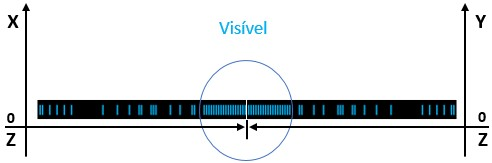
\includegraphics[scale=.4]{sections/images/consciousness_flat_universe.jpg}
	\floatfoot{Concentration of 99\% of samples.}%\footnotemark}
	\end{figure}
	%\footnotetext{Fonte: note}

\subsubsubsection{Spiral}
As the X, Y, and Z coordinates of the entangled pairs of a population tend to increase, their arrangement in a three-dimensional coordinate system will follow a diagonal reference between these three axes, as shown in Figure \ref{fig:consciousness_space_spiral_reference_line}. The observed spiral pattern does not invalidate other possible movements in space. Often, it is not possible to immediately observe the spiral pattern in the movements of an interval (subset), yet this pattern underlies many of these movements.  Taking human movements, for example, there are predominant cycles of going and coming home, going to and from work, waking up and sleeping, that is, habits are similar to movements in cycles (spiral movements).
	\begin{figure}[H]
	\caption{Three-dimensional coordinate system}
	\label{fig:consciousness_space_spiral_reference_line}
	\centering
	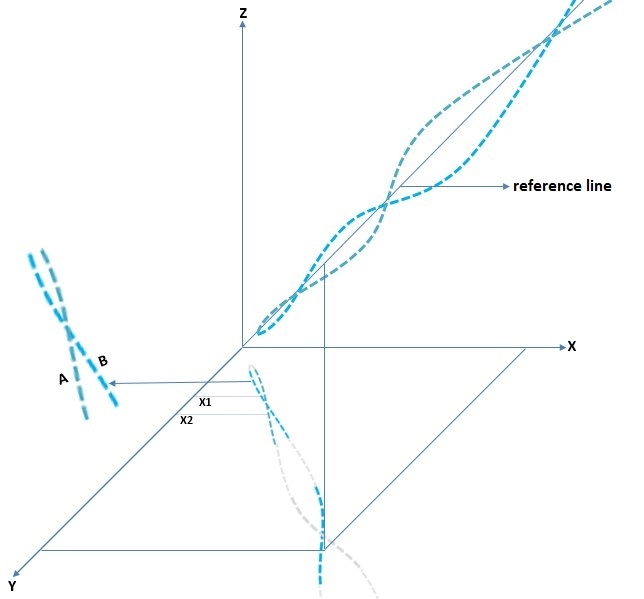
\includegraphics[scale=.6]{sections/images/consciousness_space_spiral_reference_line.jpg}
	\floatfoot{Probabilistic reference line for distribution of a population in a three-dimensional plane.}%\footnotemark}
	\end{figure}
	%\footnotetext{Fonte: note}}

In Figure \ref{fig:consciousness_space_spiral_reference_line} points X1 and X2 can also be observed. These points were mirrored in the X and Z coordinates to make it easier to observe that raising the Z axis also raises the X or Y axis, regardless of their minimum probabilistic points. The dashed lines show the most probable paths to the A and B intervals. Thus, when a part of the interval is at its maximum midpoint (X and/or Y axes) the probabilistic tendency is that it receives fewer samples than the part of the interval that is at its minimum midpoint. This spiral effect is more noticeable the larger an interval and its quantity of samples, as the more probable and stable these paths will be.

Each interval or subinterval (wavelength) has its own reference line. Just as within a meter there are centimeters, millimeters, etc., within an interval and subinterval there can be numerous other subintervals, as shown in Figure \ref{fig:consciousness_gravitational_force_system}.
	\begin{figure}[H]
	\caption{Intervals and reference lines}
	\label{fig:consciousness_space_spiral_underlines}
	\centering
	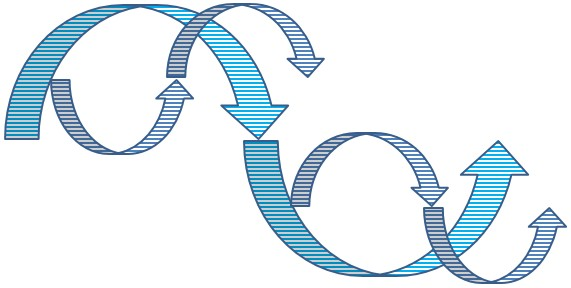
\includegraphics[scale=.5]{sections/images/consciousness_space_spiral_underlines.jpg}
	\floatfoot{Spirals at different intervals and their reference lines.}%\footnotemark}
	\end{figure}
	%\footnotetext{Fonte: note}}

\subsubsection{Fundamental forces}
The gravitational force, the electromagnetic force and the nuclear force correspond to the so-called fundamental forces of nature. These fundamental forces are not forces as such, but probabilistic aspects of population distribution and wave entanglement.

\subsubsubsection{Gravitational force}
The gravitational force is not a force itself, but an aspect of the probability distribution of new samples towards the median of the population, according to the central limit theorem.  This probabilistic direction causes waves to have a probable path to follow within the population, that is, the peak of the samples in the population or the peak of the largest wave in the population, as shown in Figures \ref{fig:consciousness_space_spiral_reference_line} and \ref{fig:consciousness_space_spiral_underlines}. Similarly, they also make the samples within a subinterval have a probable path to follow, that is, the peak of the samples in the subinterval (peak of this wave).  These sample peaks are usually the most easily observable part of a wave, since they occupy a not-so-small area.

In the Figure \ref{fig:consciousness_gravitational_force} it can be seen that the most easily observable part is slightly to the right at the peak of the wave. This wave tends to move up and to the right in a diagonal that depends on the probabilistic distribution of the new samples, as seen by the larger number of blue columns to the right of the wave (toward the median) relative to the left.
	\begin{figure}[H]
	\caption{Gravitational force}
	\label{fig:consciousness_gravitational_force}
	\centering
	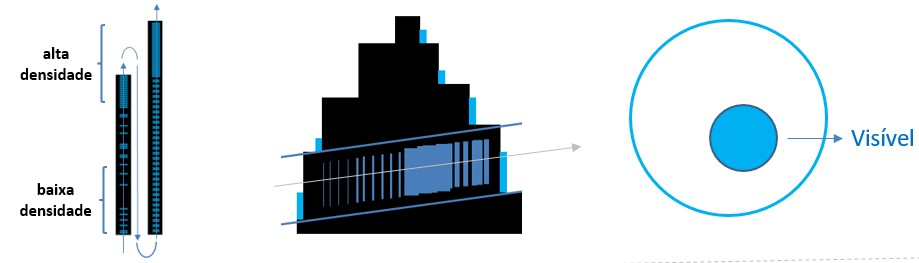
\includegraphics[scale=.7]{sections/images/consciousness_gravitational_force.jpg}
	\floatfoot{Gravitational aspect - the probabilistic direction of the distribution of new samples within an interval.}%\footnotemark}
	\end{figure}
	%\footnotetext{Fonte: note}

As seen in the Wavelength and amplitude subsection, the area of an interval grows quadratically, since the jump caused by the entanglement of the waves and the probability distribution of the samples tends to maintain an equivalent growth in the pairs that form a wave. This aspect configures the inverse square law, where, in the case of gravity, the closer the objects, the greater the probabilistic chances of new samples of the smaller object heading towards the larger object (since the larger object tends to be the peak of wave - the probabilistic direction within the wave). Thus, for being within a smaller square area and, consequently, having less possibility of movement, it ends up increasing the chances of these objects approaching with a much smaller amount of logical moments. On the other hand, the more distant the objects, the larger the area, the greater the positioning possibilities and the more logical moments are needed for the approach, featuring less attraction. Probability can also drive away more rarefied objects that should be further away from the denser and more easily observable part of a wave, as in the case of helium gas, for example. The distribution of new samples in the rarefied intervals is slower than in the denser intervals (otherwise they would not be rarefied), so these dense particles receive more samples in a shorter amount of time, occupying the front of the less dense particles.

When looking at the entire population interval, the lowest wave is the base wave of all the other sub-waves, with the population having a significant amount of samples.  Similarly, higher-level waves such as the level two in Figure \ref{fig:consciousness_gravitational_force_system} are nested within a level one wave. These systems can become much more complex in their nesting and are very common. The blue lines in the Figure below represent the probabilistic reference lines, as explained in Figure \ref{fig:consciousness_space_spiral_underlines}.
	\begin{figure}[H]
	\caption{Gravitational force - system}
	\label{fig:consciousness_gravitational_force_system}
	\centering
	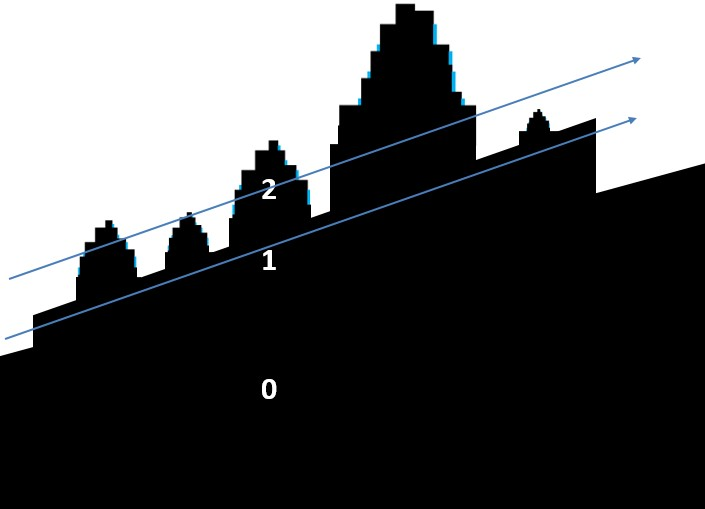
\includegraphics[scale=.4]{sections/images/consciousness_gravitational_force_system.jpg}
	\floatfoot{Gravitational aspects of a system - base wave and its sub-waves.}%\footnotemark}
	\end{figure}
	%\footnotetext{Fonte: note}
	
Figure \ref{fig:consciousness_gravitational_orbit} shows in its first example that wave 1, which could be a satellite, can rapidly approach wave 0 as new samples are distributed within the entire interval. The second example shows that the impulse the satellite receives when placed in orbit causes its wave to have a more uniform probability distribution (this uniform growth is facilitated by the low surrounding density, further away from the probabilistic peak - 1 sample in 100 is more relevant than 1 sample in 1000), where the part of the wave in blue is closer to the population median and has a growth or displacement equivalent to its lower wave, which keeps it constant. The third example is a better look at the second example, for ease of understanding, where wave 1 is defined by the spiral around the circular object representing the probabilistic peak. Perhaps the distribution of the samples at the peak, which is larger and the wave more uniform caused by the impulse (speed), can facilitate the understanding of the advance of atomic clocks on satellites.
	\begin{figure}[H]
	\caption{Gravitational force - orbit}
	\label{fig:consciousness_gravitational_orbit}
	\centering
	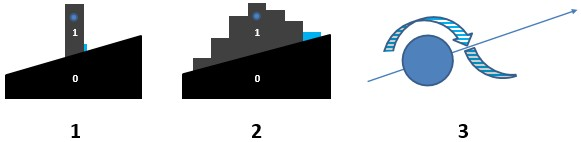
\includegraphics[scale=.9]{sections/images/consciousness_gravitational_orbit.jpg}
	\floatfoot{Gravitational aspects of a system - orbit.}%\footnotemark}
	\end{figure}
	%\footnotetext{Fonte: note}	

\subsubsubsection{Electromagnetic force}
The electromagnetic force is not a force in itself, but an aspect of the entanglement of waves that intensifies at intervals or wavelengths with low entropy and with the spatial approximation (reduction of differences in the X, Y and Z axes) of these intervals.

Electromagnetism is related to intervals similar to the more uniform wave found in the second example in Figure \ref{fig:consciousness_gravitational_orbit}, but with low entropy, that is, the same structure that facilitates the movement of objects added to the low entropy, which facilitates jumps. When intervals have low entropy, their approximation, either naturally through the structure that facilitates movement or through the distribution of new samples capable of creating this structure, such as electrification, makes the wave pairs of one interval very similar to the wave pairs of the other interval, which makes many of these pairs viable for wave entanglement to finding more ideal pairs in the other interval and vice versa. In this way, a rearrangement occurs between the intervals through wave entanglement, and this rearrangement makes these intervals more equalized (low entropy).

The blue lines in the figure \ref{fig:consciousness_electromaagnetic_force} show where the exchange of wave pairs by wave entanglement is most frequent, that is, where the waves are most probable to be similar. This is why magnets try to rotate to connect when they are face to face with the same pole. The gray line shows connections that occur in a much smaller number.
	\begin{figure}[H]
	\caption{Electromagnetic force}
	\label{fig:consciousness_electromaagnetic_force}
	\centering
	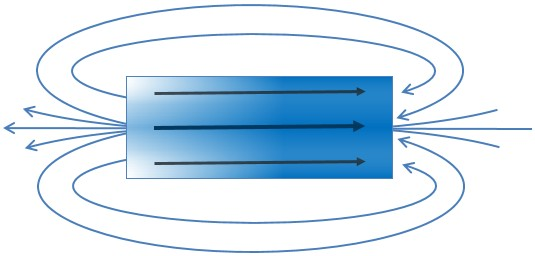
\includegraphics[scale=.7]{sections/images/consciousness_electromaagnetic_force.jpg}
	\floatfoot{Increased possibilities of wave entanglement due to probabilistic equalization in close and low entropy objects.}%\footnotemark}
	\end{figure}
	%\footnotetext{Fonte: note}

Figure \ref{fig:consciousness_electromaagnetic_force_entropy} shows an example of low entropy.
	\begin{figure}[H]
	\caption{Electromagnetic force - entropy}
	\label{fig:consciousness_electromaagnetic_force_entropy}
	\centering
	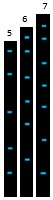
\includegraphics[scale=.9]{sections/images/consciousness_electromaagnetic_force_entropy.jpg}
	\floatfoot{Increased possibilities for wave entanglement due to low entropy.}%\footnotemark}
	\end{figure}
	%\footnotetext{Fonte: note}

The electromagnetic aspect is closely related to the low entropy of an interval and the possibility of entanglement of its pairs with surrounding pairs. The low entropy of an interval indicates that its samples are in some sort of order within it.

Probabilistically, the most similar wave pairs are found in the closest regions (blue lines in the figure \ref{fig:consciousness_electromaagnetic_force}). This occurs due to the growth of the number of samples towards the median of the population, however it is not a rule and the poles may reverse, that is, have more connections with the region of lower probability, even though most of the pairs that make up this region are increasing towards the median.

\subsubsubsection{força nuclear}
Os mesmos aspectos probabilísticos que regem a gravidade e que podem ser vistos nas Figuras \ref{fig:consciousness_gravitational_force} e \ref{fig:consciousness_gravitational_force_system} também regem as chamadas forças nucleares. A diferença é que nas forças nucleares os intervalos são menores possibilitando uma quantidade muito maior de saltos e suas ondas são mais discrepantes, conforme mostra a Figura \ref{fig:consciousness_space_subconsciousness_min}.

As forças nucleares forte e fraca representam grandes concentrações de momentos lógicos por intervalo populacional, uma alta densidade em um pequeno intervalo. A grande concentração dessas amostras está no pico do intervalo, que ocupa um subintervalo cada vez menor dentro da onda, devido à alta concentração de amostras em intervalos cada vez menores. Esses picos podem ser vistos nas Figuras \ref{fig:consciousness_dark_matter_dark_energy} e \ref{fig:consciousness_dark_matter_dark_energy_wave} e eles diminuem proporcionalmente à medida que concentram ainda mais novas amostras. Estes momentos ou amostras tendem a estarem cada vez mais juntos dentro do intervalo formando picos cada vez mais altos e densos. Esses picos são frequentemente encontrados do meio para frente dos sistemas (o núcleo ou pico do sistema), como mostrado na onda mais alta do nível dois da Figura \ref{fig:consciousness_gravitational_force_system}.

A penetração desses intervalos pequenos e densos por uma quantidade excessiva de momentos lógicos (outro intervalo semelhante), em um curto período, faz com que os inúmeros pares desses intervalos (subintervalos) se tornem muito maiores progressivamente. Dessa forma cada subintervalo salta de forma continua, progressiva e rapidamente para correspondentes cada vez maiores até que a probabilidade de destruição normalize todo o intervalo posteriormente.

\subsubsection{Matéria escura e energia escura}
A matéria e energia escuras são efeitos da observação da densidade dos intervalos, das amplitudes de ondas, conforme Figura \ref{fig:consciousness_space_volume_amplitude}. Dessa forma, intervalos maiores terão uma área facilmente observável mais ampla (picos de ondas), assim como são mais amplas suas ondas inferiores, como pode ser visto no nível zero da Figura \ref{fig:consciousness_gravitational_force_system}. Os picos de ondas se afastam por receberem uma quantidade maior de amostras, pois estão mais próximos da mediana da população e deixam as ondas inferiores cada vez menos densas em amostras, conforme Figura \ref{fig:consciousness_space_amplitude_growth}. Porém, as amostras das ondas inferiores de um grande intervalo podem ser observadas completamente a medida que os subintervalos de um intervalo são observados subsequentemente.

A gravidade ou o caminho probabilístico de um pequeno sistema ou de toda a população, o maior sistema, também pode ser visto na Figura \ref{fig:consciousness_gravitational_force_system}.

\subsubsection{Antimatéria}
Quando um intervalo tende a concentrar suas amostras sentido da mediana, o que é o sentido provável conforme teorema central do limite, dá-se o nome de matéria. A antimatéria é o contrário, quando um intervalo tende a concentrar suas amostras no sentido oposto à mediana. 

A maneira mais simples de visualizar o sentido probabilístico das amostras de qualquer comprimento de onda é observar a \textbf{linha de referência probabilística}, conforme exibido na Figura \ref{fig:consciousness_space_spiral_reference_line}. Quanto maior a quantidade de amostra de um intervalo maior será sua tendência probabilística sentido a mediana da população.

Na Figura \ref{fig:consciousness_concentration_of_opposite_samples} é exibido dois intervalos idênticos com suas amostras em concentrações opostas.
	\begin{figure}[H]
	\caption{Parte de um intervalo idêntico com suas concentrações de amostras opostas}
	\label{fig:consciousness_concentration_of_opposite_samples}
	\centering
	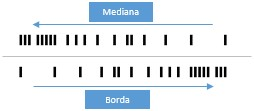
\includegraphics[scale=1.2]{sections/images/consciousness_concentration_of_opposite_samples.jpg}
	\floatfoot{Parte de um intervalo idêntico distribuídos de formas opostas.}%\footnotemark}
	\end{figure}
	%\footnotetext{Fonte: note}

O merge ou soma dos intervalos opostos da Figura \ref{fig:consciousness_concentration_of_opposite_samples} os tornaria um intervalo simétrico, ou seja, não estaria em nenhum dos sentidos.
Na Figura \ref{fig:consciousness_concentration_of_opposite_samples_within_range} é exibido uma população com suas concentrações de amostras sentido à mediana e outra com suas concentrações sentido às bordas do intervalo.
	\begin{figure}[H]
	\caption{Populações com suas concentrações de amostras opostas}
	\label{fig:consciousness_concentration_of_opposite_samples_within_range}
	\centering
	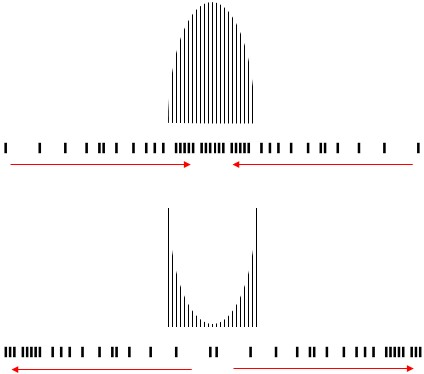
\includegraphics[scale=.7]{sections/images/consciousness_concentration_of_opposite_samples_within_range.jpg}
	\floatfoot{Populações distribuídas em sentidos contrários.}%\footnotemark}
	\end{figure}
	%\footnotetext{Fonte: note}

\subsubsection{Buraco negro}
Os buracos negros são oriundos de um aspecto probabilístico presente em qualquer intervalo da população. Esse aspecto é a alta concentração probabilísticas de amostras em intervalos cada vez menores de uma onda. O pico mais facilmente visível irá ocupar um subintervalo proporcional cada vez menor dentro do intervalo da onda, mesmo com uma concentração de amostras crescentes, conforme observado na Figura \ref{fig:consciousness_flat_universe}. Esses picos são frequentemente encontrados do meio para frente de um intervalo ou sistema (o núcleo ou pico do sistema), como mostrado na onda mais alta do nível dois da Figura \ref{fig:consciousness_gravitational_force_system}.

\subsubsection{Observador e a vida}
Os intervalos de ondas (comprimentos de ondas) que uma subconsciência (sub-lógica) é capaz de observar depende do comprimento de ondas que a própria subconsciência é constituída. Dentre todas as possibilidades de intervalos ou comprimento de ondas permitidos por uma população, o observador está em um deles. O universo não tem uma forma definida, é o observador presente em uma das possibilidades de comprimentos de onda que observa as amostras de uma população de forma condizente com seus comprimentos de ondas e com os comprimentos de ondas da população.

A capacidade de comparar ou distinguir a ordem das mudanças de uma sequência amostral é a capacidade lógica de um observador, o observador do tempo (passado e presente). A velocidade dessa observação é dada pelo range que o observador é capaz de comparar, ou seja, o qual rápido ele for capaz de distinguir pequenas mudanças (poucas amostras) o fará perceber que mudanças maiores levam mais tempo (muitas amostras). 

A capacidade lógica de fazer prospecções probabilísticas, dentro das limitações lógicas do observador e com base na probabilidade da distribuição do intervalo ou subintervalo observado é a essência do pensamento e, portanto, da vida. Essas prospecções estão fundamentadas na probabilidade de distribuição de cada intervalo (no sentido do intervalo) e, portanto, estão relacionadas com a detecção de padrão e com possibilidades probabilísticas futuras.

A capacidade de comparar ou distinguir ondas lógicas, subconjuntos ou subconsciências, é a capacidade que define o sujeito (eu). A razoabilidade dessa definição depende da proporcionalidade dessa capacidade de comparação.

A vida \underline{NÃO É}, como qualquer outra lógica. Comumente, as formas mais notáveis de vida se multiplica por estarem na média probabilística do intervalo entre seus picos e vales, por mais diferente que sejam. Porém, algo muito discrepante ou diferente do padrão médio do intervalo tende a não multiplicar e permanecer.

\subsubsubsection{Sentidos}
A parte cognitiva de uma onda não observa a si mesmo diretamente e sim o exterior (a consciência – o todo) ou mais comumente uma parte dela (a subconsciência). Essa observação pode incluir o restante da onda a qual a parte cognitiva faz parte, que também é exterior da parte cognitiva e, portanto, uma subconsciência - parte da consciência. A parte cognitiva da subconsciência humana é, provavelmente, onde se tem o maior pico de ondas do subconjunto humano. Esse é o local onde é observado a maior intensidade de mudanças. Essas mudanças são caracterizadas pelo pensamento (observação e prospecção probabilística de um intervalo) que tende ao infinito (respeitando as limitações lógicas do observador), assim como a essência da lógica, o \underline{NÃO SER}. Ou seja, a parte cognitiva é a parte que está mais próxima da observação do todo, da lógica em sua essência e totalidade, da consciência.

O universo não tem forma definida e o observador, representado na Figura \ref{fig:consciousness_amplitude_viewpoint} abaixo pelo ser humano, combina seus comprimento de ondas com os comprimento de ondas obtidos pelos sentidos, observando as formas do universo a sua maneira. A obtenção de amostras pelos sentidos os modifica e essas ondulações funcionam como ajustes ou configurações. Cada sentido observa a população amostral de forma independente, como canais de frequências distintos. Assim a visão pode estar vendo objetos muito distantes e os ouvidos escutando sons bem próximos.

Ainda na Figura \ref{fig:consciousness_amplitude_viewpoint}  pode-se observar que quanto mais largo são os objetos observados em pequenas profundidades (ponto de vista A – topo das colunas do histograma em roxo), mais fáceis esses objetos podem ser observados em maiores profundidades (ponto de vista B). É dessa forma que uma galáxia pode virar um ponto quando vista por comprimentos ou amplitudes de ondas muito grandes.
	\begin{figure}[H]
	\caption{Sentidos subconscientes - pontos de vista}
	\label{fig:consciousness_amplitude_viewpoint}
	\centering
	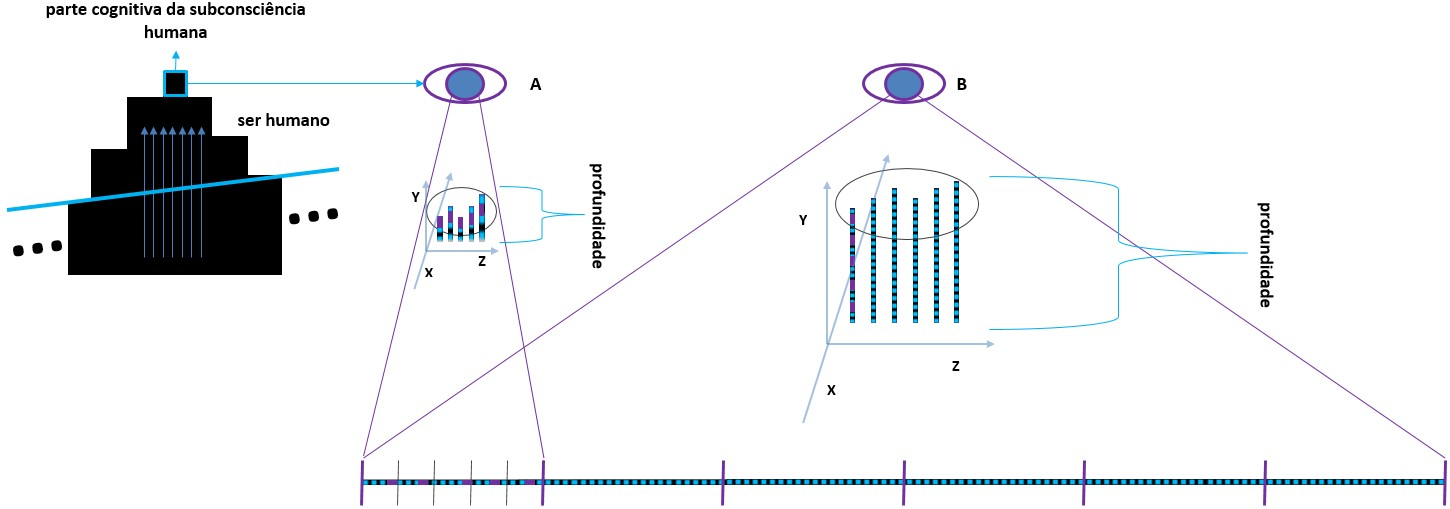
\includegraphics[scale=.4]{sections/images/consciousness_amplitude_viewpoint.jpg}
	\floatfoot{A parte cognitiva da subconsciência humana e suas observações independentes por meio dos sentidos.}%\footnotemark}
	\end{figure}
	%\footnotetext{Fonte: note}}

Na Figura acima também pode ser observado que a parte facilmente observável são os picos de ondas, definidos pelas elipses. É muito importante observar que apesar da Figura estar em 2D, o mesmo comprimento aproximado em Y pode ser visto em X, o que torna esses picos de ondas planos de observação, semelhante a gráficos de superfície.

Na Figura \ref{fig:consciousness_amplitude_crest_valley} é feita uma analogia da linha tracejada azul claro com a onda lógica do planeta Terra, por exemplo. A crista da onda é parte que recebe mais amostras e, portanto, é a parte clara e quente proveniente da luz solar (dia). Essa onda pode representa o movimento de rotação da Terra em si mesma e quando a onda humana se encontra no vale da onda do planeta, momento em que recebe menor quantidade de amostras (noite), é quando os sentidos tendem a receber menos estímulos e adormecem mais facilmente, é o adormecer da subconsciência humana.
	\begin{figure}[H]
	\caption{Crista e vale do subconjunto terrestre}
	\label{fig:consciousness_amplitude_crest_valley}
	\centering
	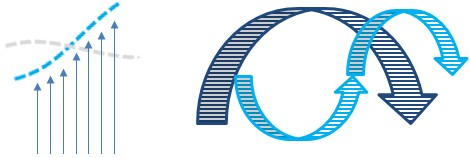
\includegraphics[scale=.6]{sections/images/consciousness_amplitude_crest_valley.jpg}
	\floatfoot{Crista e vale terrestre como característica do adormecimento dos sentidos humanos.}%\footnotemark}
	\end{figure}
	%\footnotetext{Fonte: note}}

Uma característica importante do processo de observação de pequenos intervalos é que eles podem ser observados com partículas ou ondas, conforme Figura \ref{fig:consciousness_space_wave-particle}. Nessa Figura é contemplado um pequeno intervalo, análogo a um fóton, como exemplo. Na observação como partícula o observador acompanha um intervalo representado por um par entrelaçado, observando sua forma e movimento consistentes no espaço. No efeito partícula, a consistência da forma e seus movimentos são estabelecidas pelo par entrelaçado, visto que o salto ocorre em um lado do par de cada vez, garantido estabilidade nas mudanças.

Na Figura abaixo também é contemplado o intervalo observado como onda, onde o observador fixa em um intervalo representado por uma das partes que compõe pares entrelaçados e acompanha seus movimentos e saltos, uma vez que os saltos são frequentes em pequenos intervalos. A adição de novas amostras na população faz com que ela se distribua proporcionalmente para acoplar essas novas amostras, o que movimenta as amostras deste pequeno intervalo, conforme visto na Figura \ref{fig:consciousness_space_volume_amplitude}. No efeito de onda, os movimentos saltam e transitam entre picos e vales com altas frequências ou vibrações devido ao pequeno tamanho do intervalo e aos saltos provocados pelas novas amostras dentro desse intervalo e pelas mudanças feitas pela distribuição proporcionalmente de novas amostras na população.
	\begin{figure}[H]
	\caption{Observador - onda-partícula}
	\label{fig:consciousness_space_wave-particle}
	\centering
	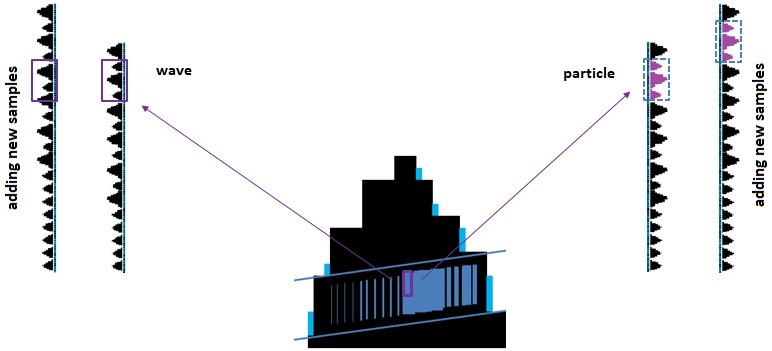
\includegraphics[scale=.55]{sections/images/consciousness_space_wave-particle.jpg}
	\floatfoot{Características da observação de uma pequena parte de um subconjunto.}%\footnotemark}
	\end{figure}
	%\footnotetext{Fonte: note}}

Talvez não seja possível observar o efeito onda sem entrelaçar seu par. A alta frequência desse intervalo faz com que ele ocupe ou transite rapidamente em uma área ao seu redor, o que pode facilitar o colapso da onda em um ponto especifico e então observar o seu efeito partícula (semelhante ao olho humano) ou em um local mais amplo e observar seu efeito onda com o colapso de muitas amostragens.
